\documentclass[10pt,t,xcolor=dvipsnames]{beamer}

\usetheme{Antibes}
\usecolortheme{structure}
%\usepackage[utf8x]{inputenc}
%\usepackage{default}
%\usecolortheme{albatross}
%\usecolortheme{lily}
%\usecolortheme{sidebartab}
%\usecolortheme{crane}
%\usecolortheme{orchid}
%\usecolortheme{albatross}
%\usecolortheme{beetle}
%\usecolortheme{dove}
%\usecolortheme{fly}
%\usecolortheme{seagull}
%\usecolortheme{dolphin}
%\usecolortheme{rose}
\usepackage{graphics}
% \usepackage[pdftex]{graphicx}
\usepackage{graphicx}
\usepackage{xcolor}
\usepackage{color}
%\usepackage{url}
\usepackage{hyperref}
%\usepackage[obeyspaces]{url}
\usepackage{amssymb,amsmath} % for the bold symbol command
\usepackage{booktabs} % toprule etc in tables
\usepackage{mathrsfs}
\usepackage{listings}
\lstset{ %
  backgroundcolor=\color{white},
  basicstyle=\footnotesize,
  breakatwhitespace=false,
  breaklines=true,
  captionpos=b,
  commentstyle=\color{green},
  escapeinside={\%*}{*)},
  extendedchars=true,
  frame=single,
  keywordstyle=\color{blue},
  language=bash,
  numbers=left,
  numbersep=5pt,
  numberstyle=\tiny\color{gray},
  rulecolor=\color{black},
  showspaces=false,
  showstringspaces=false,
  showtabs=false,
  stepnumber=2,
  stringstyle=\color{red},
  tabsize=2,
  title=\lstname,
  morekeywords={not,\},\{,preconditions,effects },
  deletekeywords={time}
}
%\usepackage{minted}
%\usepackage{beamerthemebars}
%\usepackage{ragged2e}
%\usepackage{lipsum}

\setbeamercolor{structure}{fg=MidnightBlue!50!black}
\renewcommand{\raggedright}{\leftskip=0pt \rightskip=0pt plus 0cm}
\logo{
\includegraphics[scale=0.05]{../../../TWAssets/TW_Colour_Logos_trans_green.png}}

\title{ An Introduction to Django }
\titlegraphic{
\includegraphics[scale=0.15]{../../../TWAssets/TW_Colour_Logos_trans_green.png}}

\author{ Patrick Turley \& 'Wole Solana }
\begin{document}
\nocite*{}
\frame [c, plain]{\titlepage}
%-------------------------------Slide1-------------------------------
\section{Introduction}
\begin{frame}
\frametitle{What is Django?}
\pause
\begin{columns}[l]
\column{0.5\textwidth}
\begin{itemize}[<+->]
\item \alert{Django} is an open source web application (web app) framework written in Python, and follows the \alert{Model-View-Controller} (MVC) design pattern.
\item A \alert{web framework} can be loosely defined as a set of components that assist in building web apps faster and easier.
\item Other frameworks include Rails (Ruby), Drupal (PHP) and Spring (Java)
\item Popular sites built with Django include NASA, Instagram, The Guardian.
\end{itemize}
\column{0.5\textwidth}
\begin{figure}
\centering

\includegraphics[scale=0.3]{../images/django.jpg}
\end{figure}
\end{columns}
\end{frame}
%------------------------------Slide2---------------------------------
\begin{frame}[fragile]
\frametitle{Why use a web framework?}
\pause
\begin{columns}[l]
\column{0.5\textwidth}
\vspace{-1cm}
\begin{figure}
\centering
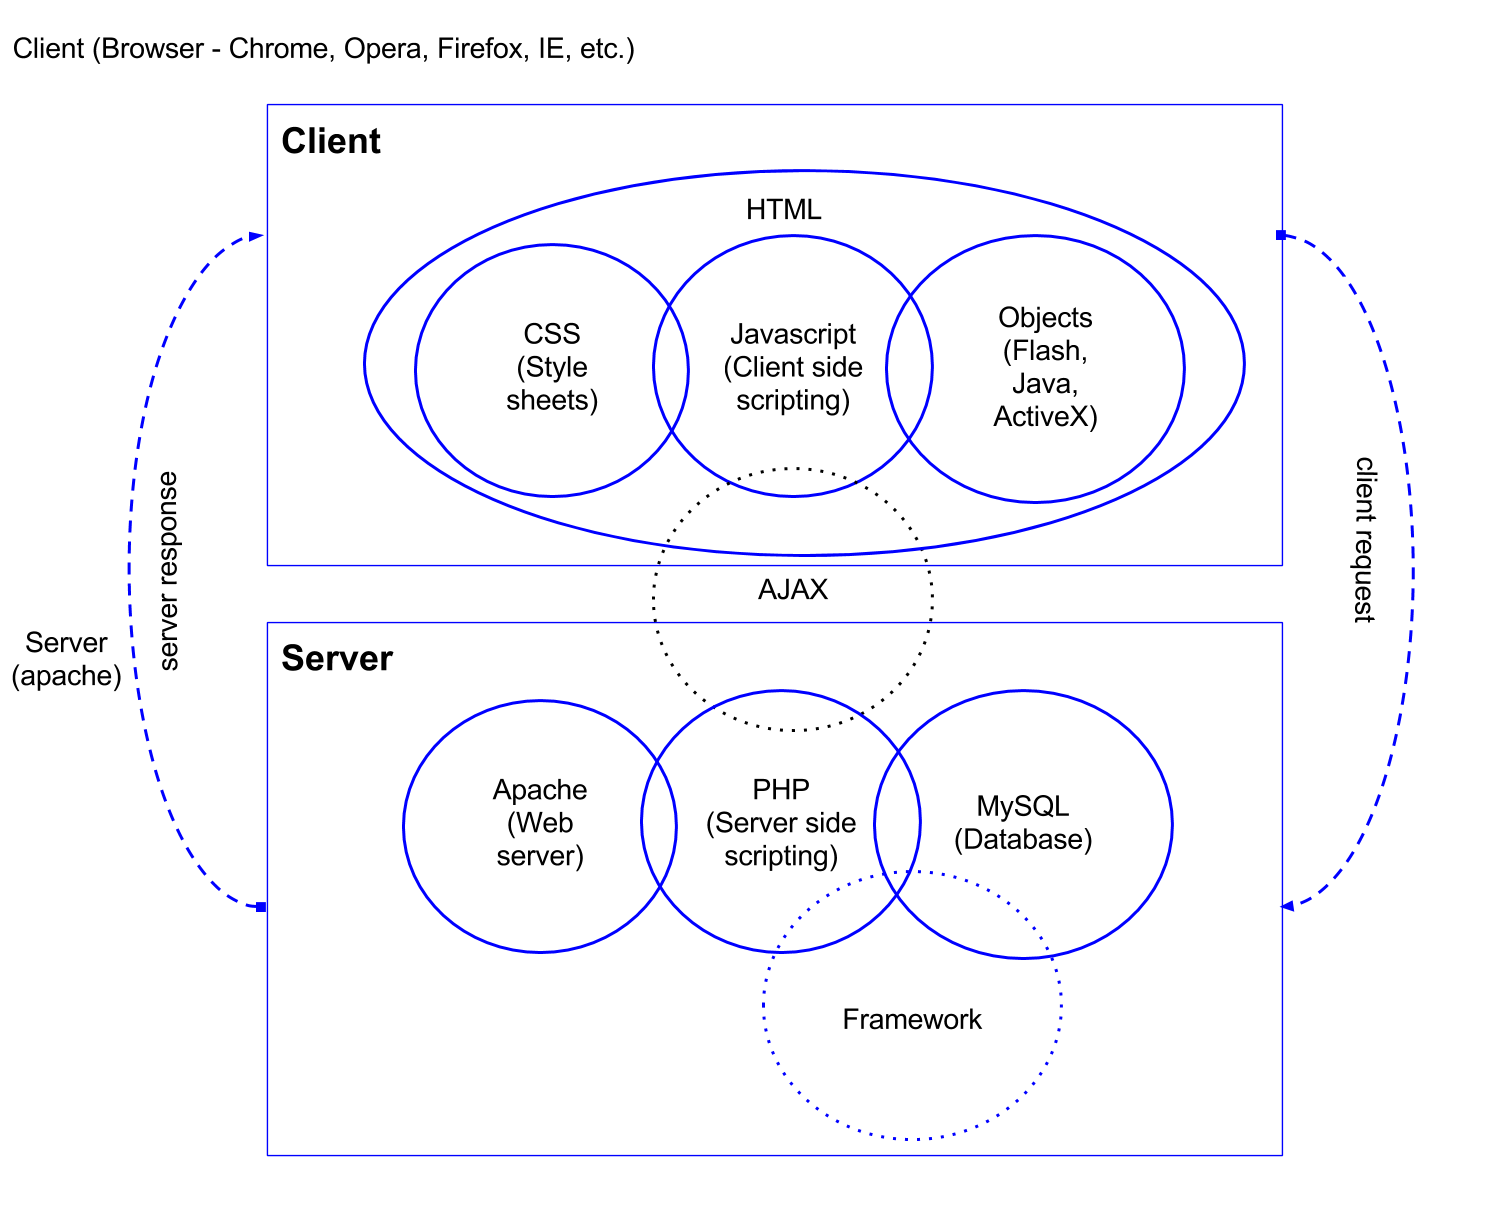
\includegraphics[scale=0.125]{../images/webapp_building_blocks.png}
\caption{\footnotesize{Schematic diagram of a web app}}
\end{figure}
\column{0.5\textwidth}
\begin{itemize}[<+->]
\item It enables us to build web apps faster by focusing on the unique functionality of our web app rather than the infrastucture
\item Most provide us with with libraries and templates which we can reuse, thus enhancing our productivity.
\end{itemize}
\end{columns}
\end{frame}
%------------------------------Slide3----------------------------------
\section{The MVC design paradigm}
\begin{frame}[fragile]
\frametitle{Model-View-Controller}
\pause
\begin{columns}[l]
\column{0.4\textwidth}
\begin{itemize}[<+->]
\item A design pattern (which extends OOP) that helps us better organise our web app by \alert{separating concerns}
\item The \textbf{model} contains \alert{data and logic}, the \textbf{view} forms the \alert{user interface} (what the user sees) and the \textbf{controller} manages the \alert{interaction} between the model and view.
\end{itemize}
\column{0.5\textwidth}
\vspace{-0.5cm}
\begin{figure}
\hspace*{-0.5cm}
\centering
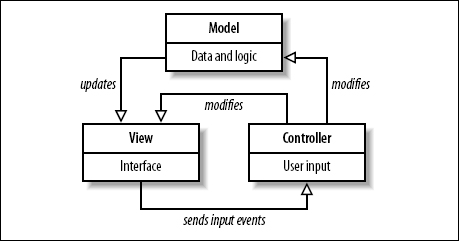
\includegraphics[scale=0.4]{../images/mvc-02.jpg}
\caption{The MVC pattern}
\end{figure}
\end{columns}
\end{frame}
%--------------------------------------------Slide7------------------------------------------------------------------
\section{Our first Django app}
\begin{frame}[fragile]
\frametitle{Installation and set up}
\begin{itemize}[<+->]
\item Setup your virtual environment
\begin{lstlisting}
virtualenv django_env
\end{lstlisting}
\item Activate your virtual environment
\begin{lstlisting}
source django_env/bin/activate
\end{lstlisting}
\item Install django
\begin{lstlisting}
pip install django
\end{lstlisting}
\item Start your project
\begin{lstlisting}
django-admin startproject first_site
\end{lstlisting}
\end{itemize}
\end{frame}
%--------------------------------------------Slide8------------------------------------------------------------------
\begin{frame}[fragile]
\frametitle{Let's take a look at our app}
\begin{itemize}[<+->]
\item Setup the database. Go into the \texttt{firstsite} folder and run
\begin{lstlisting}
python manage.py migrate
\end{lstlisting}
\item Run the server
\begin{lstlisting}
python manage.py runserver &
\end{lstlisting}
\item In your browser, navigate to \texttt{http://127.0.0.1:8000/}, and \textit{voila!}
\end{itemize}
\end{frame}
%--------------------------------------------Slide9------------------------------------------------------------------
\begin{frame}[fragile]
\frametitle{Let's add some content}
\begin{itemize}[<+->]
\item Still in the \texttt{firstsite} folder, run
\begin{lstlisting}
python manage.py startapp my_library
\end{lstlisting}
\item Open the \texttt{settings.py} file and in the file, add `\texttt{my\_library}' to the \texttt{INSTALLED\_APPS} list so you have something like this:
\begin{verbatim}
INSTALLED_APPS = (
    `django.contrib.admin',
    `django.contrib.auth',
    `django.contrib.contenttypes',
    `django.contrib.sessions',
    `django.contrib.messages',
    `django.contrib.staticfiles',
    `my_library',
)
\end{verbatim}
\end{itemize}
\end{frame}
%--------------------------------------------Slide10------------------------------------------------------------------
\begin{frame}[fragile]
\frametitle{Creating the book model}
\begin{itemize}[<+->]
\item Open \texttt{my\_library/models.py}
\item Edit the file (we'll do this together) with the model attributes
\item Update the database
\begin{lstlisting}
python manage.py makemigrations my_library
python manage.py migrate my_library
\end{lstlisting}
\item Open the \texttt{my\_library/admin.py} file. Update it with the following content:
\begin{verbatim}
from django.contrib import admin
from my_library.models import Book
admin.site.register(Book)
\end{verbatim}
\item In your browser, visit `\texttt{http://127.0.0.1:8000/admin}'
\end{itemize}
\end{frame}
%--------------------------------------------Slide11------------------------------------------------------------------
\begin{frame}[fragile]
\frametitle{Some admin}
\begin{itemize}[<+->]
\item Create a superuser
\begin{lstlisting}
python manage.py createsuperuser
python manage.py migrate my_library
\end{lstlisting}
\item Go back to `\texttt{http://127.0.0.1:8000/admin}', log in and create some books
\end{itemize}
\end{frame}
%--------------------------------------------Slide12------------------------------------------------------------------
\begin{frame}[fragile]
\frametitle{So how do we get to see our view?}
%\begin{itemize}[<+->]
%\end{itemize}
\end{frame}
%--------------------------------------------Slide13------------------------------------------------------------------
%\section{Further Reading}
%\begin{frame}
%\frametitle{Further Reading}
%% \bibliographystyle{plain}
%% \bibliography{DevelopmentPractices.bib}
%\end{frame}
\end{document}
